% -*- latex -*-

%%%%%%%%%%%%%%%%%%%%%%%%%%%%%%%%%%%%%%%%%%%%%%%%%%%%%%%%%%%%%%%%%%%%%%%%%%%%%
% This beginning part of the preamble is specific to the vgtc document class.

\documentclass{vgtc}                          % final (conference style)
%\documentclass[review]{vgtc}                 % review
%\documentclass[widereview]{vgtc}             % wide-spaced review
%\documentclass[preprint]{vgtc}               % preprint
%\documentclass[electronic]{vgtc}             % electronic version

%% Uncomment one of the lines above depending on where your paper is
%% in the conference process. ``review'' and ``widereview'' are for review
%% submission, ``preprint'' is for pre-publication, and the final version
%% doesn't use a specific qualifier. Further, ``electronic'' includes
%% hyperreferences for more convenient online viewing.

%% Please use one of the ``review'' options in combination with the
%% assigned online id (see below) ONLY if your paper uses a double blind
%% review process. Some conferences, like IEEE Vis and InfoVis, have NOT
%% in the past.

%% Figures should be in CMYK or Grey scale format, otherwise, colour 
%% shifting may occur during the printing process.

%% These three lines bring in essential packages: ``mathptmx'' for Type 1 
%% typefaces, ``graphicx'' for inclusion of EPS figures. and ``times''
%% for proper handling of the times font family.

\usepackage{mathptmx}
\usepackage{graphicx}
\usepackage{times}

%% We encourage the use of mathptmx for consistent usage of times font
%% throughout the proceedings. However, if you encounter conflicts
%% with other math-related packages, you may want to disable it.

%% If you are submitting a paper to a conference for review with a double
%% blind reviewing process, please replace the value ``0'' below with your
%% OnlineID. Otherwise, you may safely leave it at ``0''.
\onlineid{6}

%% declare the category of your paper, only shown in review mode
\vgtccategory{Research}

%% allow for this line if you want the electronic option to work properly
\vgtcinsertpkg

%% In preprint mode you may define your own headline.
%\preprinttext{To appear in an IEEE VGTC sponsored conference.}

%% Paper title.

\title{A Proposed Framework for Data Analysis and Visualization at Extreme Scale}

%% This is how authors are specified in the conference style

%% Author and Affiliation (single author).
%%\author{Roy G. Biv\thanks{e-mail: roy.g.biv@aol.com}}
%%\affiliation{\scriptsize Allied Widgets Research}

%% Author and Affiliation (multiple authors with single affiliations).
%%\author{Roy G. Biv\thanks{e-mail: roy.g.biv@aol.com} %
%%\and Ed Grimley\thanks{e-mail:ed.grimley@aol.com} %
%%\and Martha Stewart\thanks{e-mail:martha.stewart@marthastewart.com}}
%%\affiliation{\scriptsize Martha Stewart Enterprises \\ Microsoft Research}

%% Author and Affiliation (multiple authors with multiple affiliations)
%% \author{Roy G. Biv\thanks{e-mail: roy.g.biv@aol.com}\\ %
%%         \scriptsize Starbucks Research %
%% \and Ed Grimley\thanks{e-mail:ed.grimley@aol.com}\\ %
%%      \scriptsize Grimley Widgets, Inc. %
%% \and Martha Stewart\thanks{e-mail:martha.stewart@marthastewart.com}\\ %
%%      \parbox{1.4in}{\scriptsize \centering Martha Stewart Enterprises \\ Microsoft Research}}

\author{
  Utkarsh Ayachit\thanks{email: utkarsh.ayachit@kitware.com} \\ %
  \scriptsize Kitware, Inc. %
  \and %
  Kenneth Moreland\thanks{email: kmorel@sandia.gov} \\ %
  \scriptsize Sandia National Laboratories %
  \and %
  Berk Geveci\thanks{email: berk.geveci@kitware.com} \\ %
  \scriptsize Kitware, Inc. %
  \and %
  Kwan-Liu Ma\thanks{email: ma@cs.ucdavis.edu} \\ %
  \scriptsize University of California at Davis %
}

%% A teaser figure can be included as follows, but is not recommended since
%% the space is now taken up by a full width abstract.
%\teaser{
%  \includegraphics[width=1.5in]{sample.eps}
%  \caption{Lookit! Lookit!}
%}

%% Abstract section
\abstract{ Experts agree that the exascale machine will comprise processors
  that contain many cores, which in turn will necessitate a much higher
  degree of concurrency.  Software will require a minimum of a 1000 times
  more concurrency.  Most parallel analysis and visualization algorithms
  today work by partitioning data and running mostly serial algorithms
  concurrently on each data partition.  Although this approach lends itself
  well to the concurrency of current high performance computing, it does
  not exhibit the appropriate pervasive parallelism required for exascale
  computing. The data partitions are too small and the overhead of the
  threads too large to make effective use of all the cores in an extreme
  scale machine.  This paper introduces a new visualization framework
  designed to exhibit the pervasive parallelism necessary for extreme scale
  machines.  We demonstrate the use of this system on a GPU processor,
  which we feel is the best analog to an exascale node that we have
  available today.  }

%% ACM Computing Classification System (CCS). 
%% See <http://www.acm.org/class/1998/> for details.
%% The ``\CCScat'' command takes four arguments.

\CCScatlist{
  \CCScat{D.1.3}{Software}{Programming Techniques}{Concurrent Programming}
}

%% Copyright space is enabled by default as required by guidelines.
%% It is disabled by the 'review' option or via the following command:
% \nocopyrightspace

% End of vgtc-specific portion of the preamble.
%%%%%%%%%%%%%%%%%%%%%%%%%%%%%%%%%%%%%%%%%%%%%%%%%%%%%%%%%%%%%%%%%%%%%%%%%%%%%

\usepackage{amsfonts}
\usepackage{amssymb}
\usepackage{amsmath}
\usepackage{graphicx}
\usepackage{varioref}
\usepackage{fancyvrb}
\usepackage{ifthen}
\usepackage{cite}
\usepackage{subfigure}
\usepackage{xspace}
%\usepackage{hyperref}

\usepackage{color}
\definecolor{yellow}{rgb}{1,1,0}
\definecolor{black}{rgb}{0,0,0}
\definecolor{ltcyan}{rgb}{.75,1,1}
\definecolor{red}{rgb}{1,0,0}

% Cite commands I use to abstract away the different ways to reference an
% entry in the bibliography (superscripts, numbers, dates, or author
% abbreviations).  \scite is a short cite that is used immediately after
% when the authors are mentioned.  \lcite is a full citation that is used
% anywhere.  Both should be used right next to the text being cited without
% any spacing.
\newcommand*{\lcite}[1]{~\cite{#1}}
\newcommand*{\scite}[1]{~\cite{#1}}

\newcommand*{\keyterm}[1]{\emph{#1}}

\newcommand{\etal}{et al.}

\newcommand{\fix}[1]{{\color{red}\textbf{\textsc{[#1]}}}}

\begin{document}

%% VGTC-specific:
%% The ``\maketitle'' command must be the first command after the
%% ``\begin{document}'' command. It prepares and prints the title block.

%% the only exception to this rule is the \firstsection command
\firstsection{Introduction}

\maketitle

%% \section{Introduction} 
\label{sec:Introduction}

Most of today's visualization libraries and applications are based off of
what is known as the \keyterm{visualization
  pipeline}\lcite{Haeberli88,Lucas92}.  The visualization pipeline is the
key metaphor in many visualization development systems such as the
Visualization Toolkit (VTK)\lcite{VTKBook}, SCIRun\lcite{SCIRunPaper}, the
Application Visualization System (AVS)\lcite{AVSPaper},
OpenDX\lcite{OpenDXPaper}, and Iris Explorer\lcite{IRISExplorerPaper}.  It
is also the internal mechanism or external interface for many end-user
visualization applications such as ParaView\lcite{ParaViewGuideBook},
VisIt\lcite{VisItBook}, VisTrails\lcite{VisTrailsPaper},
MayaVi\lcite{MayaViPaper}, VolView\lcite{VolViewBook},
OsiriX\lcite{OsiriXPaper}, 3D Slicer\lcite{3DSlicerPaper}, and
BioImageXD\lcite{BioImageXDPaper}.

In the visualization pipeline model, algorithms are encapsulated as
\keyterm{filter} components with inputs and outputs.  These filters can
be combined by connecting the outputs of one filter to the inputs of
another filter.  The visualization pipeline model is popular because it
provides a convenient abstraction that allows users to combine algorithms
in powerful ways.

Although the visualization pipeline lends itself well to the concurrency of
current high performance
computing\lcite{Moreland08,Patchett09,Pugmire08,White05}, its structure
prohibits the necessary extreme concurrency required for exascale
computers.  This paper describes the design of the \keyterm{Dax toolkit} to
perform Data Analysis at Extreme scales.  The computational unit of this
framework is a \keyterm{worklet}, a single operation on a small piece of data.
Worklets can be combined in much the same way as filters, but their light
weight, lack of state, and small data access make them more suitable for
the massive concurrency required by exascale computers and associated
multi- and many-core processors.
Figure~\ref{fig:DaxPipelineVsTraditionalPipeline} highlights the difference
between a Dax pipeline
execution with a traditional visualization pipeline provided by existing
visualization frameworks such as VTK.

\begin{figure}
  \centering
  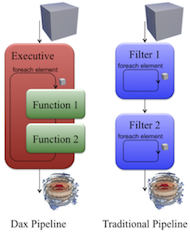
\includegraphics[width=2.5in]{images/DaxPipelineVsTraditionalPipeline}
  \caption{Comparison between Dax pipeline execution and traditional
    visualization pipeline execution. Dax makes it possible to achieve higher
    degree of concurrency by moving the iteration over mesh elements out of the
    algorithm and letting the framework manage the parallelism.
    \fix{Need highres image}}
  \label{fig:DaxPipelineVsTraditionalPipeline}
\end{figure}

\section{Related Work}
\label{sec:RelatedWork}

Since its inception, many improvements have been made to the visualization
pipeline to allow it to function well with large data.  By dividing tasks,
pipelines, or data amongst processes, the serial algorithms of a
visualization pipeline can work in parallel with little or no
modification\lcite{Ahrens00}.  In particular, the data parallel
mode, partitioning the data and replicating the pipeline, performs
well on current high performance computers\lcite{Cedilnik06}.

The basic function of a visualization pipeline is to process data flowing
from upstream to downstream.  More recent visualization pipeline
implementations, such as those in VTK, ParaView, and VisIt, implement more
advanced control mechanisms and pass meta-data throughout the pipeline.
These control mechanisms can, for example, subset the data in
space\lcite{Childs05} or time\lcite{Biddiscombe07} based on the needs of
the individual computing units.  Recent work is coupling this mechanism
with query-driven visualization techniques\lcite{Gosink08} to better sift
through large data sets with limited resources.

These control mechanisms can also be used to stream data, in pieces,
through the pipeline\lcite{Ahrens01}.  More recent advances allow us to
prioritize the streaming, thus allowing to compensate for high latency of
streaming by presenting the most relevant data first\lcite{Ahrens07}.  This
in turn has lead to multi-resolution
visualization\lcite{Pascucci01,Woodring09}.  Multiple resolutions further
hide limited resource latency by first presenting low-detailed results and
then iteratively refining them as needed.  This assumes, of course, that a
multi-resolution hierarchy of data is already built (a non-trivial task for
unstructured data).  This work is being implemented in a traditional
visualization pipeline, but could be leveraged in many other types of
frameworks, including the one proposed for this project.

Another recent research project extends the visualization-pipeline
streaming mechanism by automatically orchestrating task concurrency in
independent components of the pipeline\lcite{Vo09}.  The technique adapts
the visualization pipeline to multi-core processors, but it has its
limitations.  There is a high overhead with regard to each execution thread
created; they require isolated buffers of memory for input and output and
independent call stacks, which typically run many calls deep.  Furthermore,
algorithms in the filters are optimized to iterate over sizable data
chunks, which will not be the case with massive multi-threading.  At some
point the algorithms will have to be reengineered to process small data
chunks or themselves be multithreaded.  It will be necessary to leverage a
threading paradigm like the one proposed for this project to engineer this
kind of change on a full-featured toolkit.

An alternative data analysis and visualization architecture is implemented
by the Field Encapsulation Library (FEL)\lcite{FELPaper}.  FEL provides
abstractions that allows programs to access the structure and fields of a
mesh independently from the data storage.  More importantly, FEL uses C++
template constructs to build functional definitions of fields.  These
fields compute values on demand when requested.  These functional fields
are similar in nature to the worklets defined in our work.

Although the main concerns addressed by FEL, mesh flexibility and memory
overhead, is complementary to this project, FEL does not adequately manage
the complexity of massive multi-threading.  To support pervasive parallelism
we need to hide the complexity of work distribution.  Also, as the name
implies, the Field Encapsulation Library is primarily concerned with
defining, accessing, and operating on fields.  There is no mechanism for
topological operations that change or create meshes.  Nor is there any
explicit method for aggregation.  In order to address the varied data
analysis and visualization needs, this project enables these features.

Another system with constructs similar to the framework proposed for this
project is provided by Intel Threading Building Blocks (TBB)\lcite{TBB}, a
popular open-source C++ library for multi-core programming.  In addition to
high-level parallel constructs such as parallel looping and reduction
operations, TBB also provides a simple pipeline execution environment.
Like Dax, TBB's pipeline mechanism
partitions data based on available hardware threads, handing-off the
resulting partitions to caller-supplied functions that each iterate over
their assigned ranges to perform computation.  Thus, TBB provides a hybrid
abstraction where callers are isolated from some of the complexity of
scheduling work across multiple cores, but each function is still
responsible for iteration over its subset of the data.

This approach is appropriate for current architectures where an individual
host has a relatively small number of hardware threads, but requires that
function authors continue to deal with data organization and iteration
issues on an ad-hoc basis.  Further, TBB does not address issues of
scheduling or communication across multiple hosts in a distributed
platform.  Dax envisions a stricter separation of
responsibilities where worklets are responsible for computation only,
leaving data retrieval and inter-processor communication to separate
executive components.

The MapReduce programming model\lcite{MapReduce} is also similar in spirit
to our proposed framework.  Like our approach, MapReduce simplifies
parallel programming by defining algorithms in terms of local, stateless
operations.  However MapReduce, not being designed as such, does not have
all the conventions necessary for a fully featured visualization and data
analysis library.  For example, expressing local topological connections
(e.g. cells connected to vertices, vertices connected to cells, or cells
connected to cells) are difficult to express.  The combining of predefined
computation units is not directly supported, nor is the specification of
topological, spatial, or temporal domains.  In contrast, our proposed
system provides the primitives with which visualization and data analysis
programmers are accustomed.

\section{Motivation}
\label{sec:Motivation}


As the scale of supercomputers has progressed from the teraflop to the
petaflop we have enjoyed a resiliency of the message passing model
(embodied in the use of MPI) as an effective means of attaining
scalability.  However, as we consider the high performance computer of the
future, the exascale machine, we discover that this concurrency model will
no longer be sufficient.  All industry trends infer that the exascale
machine will be built using many-core processors containing hundreds to
thousands of cores per chip.  This change in processor design has dramatic
effects on the design of large-scale parallel programs.  As stated by a
recent study by the DARPA Information Processing Techniques
Office\lcite{DARPAExascaleStudy}:

\begin{quote}
  The concurrency challenge is manifest in the need for software to expose
  at least 1000$\times$ more concurrency in applications for Extreme Scale
  systems, relative to current systems. It is further exacerbated by the
  projected memory-computation imbalances in Extreme Scale systems, with
  Bytes/Ops ratios that may drop to values as low as $10^{-2}$ where Bytes
  and Ops represent the main memory and computation capacities of the
  system respectively. These ratios will result in 100$\times$ reductions
  in memory per core relative to Petascale systems, with accompanying
  reductions in memory bandwidth per core.  Thus, a significant fraction of
  software concurrency in Extreme Scale systems must come from exploiting
  more parallelism within the computation performed on a single datum.
\end{quote}

Put simply, efficient concurrency on exascale machines requires a massive
amount of concurrent threads, each performing many operations on a small
and localized piece of data.

Other studies concur.  The Workshop on Visual Analysis and Data Exploration
at Extreme Scale\lcite{VisAnalysisExtremeScale} corroborates the need for
``pervasive parallelism'' throughout visual analysis tools and that data
access is a prime consideration for future tools.  The International
Exascale Software Project's recent road map\lcite{ExascaleRoadMap} also
states a required thousand fold increase in concurrency and that
applications may require ten billion threads.  The road map also notes a
change in I/O and Memory that will ``affect programming models and
optimization.''  Careful consideration of memory access is also expected
to have a dramatic effect on energy consumption as much of the power of an
exascale system will be expended moving data.

Will visualization systems need to run on these exascale systems?  They
undoubtedly will.  Although it has been a common practice to use specialty
high performance platforms for visualization and graphics~\lcite{Wylie01},
this trend is coming to an end.  The cost of creating specialty
visualization computers that are capable of analyzing data generated from
large supercomputer runs is becoming prohibitive\lcite{Childs07}.
Consequently, researchers are beginning to leverage the same supercomputers
used for creating the data\lcite{Peterka09:SC,Peterka09:SciDAC,Yu08}.
This, coupled with a renewed interest in running visualization
\emph{in-situ} with simulations to overcome file I/O
constraints\lcite{SNL092014,Tu06,Ross08}, ensures that high performance
visualization code will run on the same technology as the simulation code
for the foreseeable future.

Visualization pipelines fit poorly into this massive concurrency model; the
granularity of the pipeline computational unit, the filter, is too large.
Each filter must ingest, process, and produce an entire data set when
invoked.  Large scale concurrency today is achieved by replicating the
pipeline and partitioning the input data amongst processes\lcite{Ahrens00}.
However, extreme scale computers would require the data to be broken into
billions of partitions.  The overhead of capturing the connectivity
information between these partitions as well as the overhead of executing
these large computation units on such small partitions of data is too great
to make such an approach practical.

To understand why, consider the sobering comparison between the
Jaguar XT5 partition, a current petascale machine, and the projections for
an exascale machine of by the International Exascale Software Project
RoadMap\lcite{ExascaleRoadMap} given in Table~\ref{table:PetaExaCompare}.
Because processor clock rates are not increasing, an exascale computer
requires a thousand-fold increase in the number of cores.  Furthermore,
trends in processor design suggest that these cores must be hyper-threaded
in order to keep them executing at full efficiency.  In all, to drive a
complete exascale machine will require between one and ten billion
concurrently running threads.

\begin{table}[htbp]
  \centering
  \caption{Comparison of characteristics between petascale and projected
    exascale machines.}
  \label{table:PetaExaCompare}
  \begin{tabular}{llll}
    & Jaguar -- XT5 & Exascale & Increase \\
    \hline
    Cores & 224,256 & \parbox{.7in}{\vspace*{2pt}100 million\\ \hspace*{6pt} -- 1 billion\vspace*{2pt}} & $\sim{}1,000\times$ \\
    Threads & 224,256 way & 1 -- 10 billion way & $\sim{}50,000\times$ \\
    Memory & 300 Terabytes & 128 Petabytes & $\sim{}500\times$
  \end{tabular}
\end{table}

Most of our current tools rely on MPI for concurrency.  An MPI process has
the overhead of a running program with its own memory space.  A common
process has an overhead of about twenty megabytes.  Running on the entirety
of Jaguar yields an overhead of about 4 terabytes, less than two percent of
the overall available memory.  In contrast, the overhead for using MPI
processes for all the concurrency on an exascale machine requires up to 200
petabytes, possibly exceeding the total memory on the system in overhead
alone.

Even getting around problems with the overhead of MPI, the visualization
pipeline still has inherent problems at this level of concurrency.
Consider using Jaguar to process a one trillion cell mesh.  If we partition
these cells evenly amongst all the cores where replicated pipelines will
process each partition, that yields roughly 5 million cells per pipeline.
General rules of thumb indicate this ratio is optimal for structured grids
when running parallel VTK pipelines\lcite{ParaViewTutorial}.  Scaling to an
exascale machine, we can project to processing 500 trillion cells
(considering this is the expected growth in system memory).  If we
partition these cells evenly amongst all the necessary cores where
replicated pipelines will process each partition, that yields as few as 50
thousand cells per pipeline.  Here we are starving our pipeline.

Even if we somehow avoid the problem of running on the largest exascale
machines, the problem of a fundamental change in processor architecture
persists.  The parallel visualization pipeline simply does not conform well
to multi-core processors and many-core accelerators.  In response several
researchers are pursing the idea of a \keyterm{hybrid parallel
  pipeline}\lcite{Camp10,Howison11,Li08}.  The hybrid parallel pipeline
breaks the problem into two hierarchical levels.  The first level
partitions the data amongst distributed memory nodes in the same way as the
current parallel pipeline.  In the second level we run a threaded shared
memory algorithm to take advantage of a multi- or many-core processor.

Although the current visualization pipeline does a good job in providing
this first level of distributed memory concurrency, it provides no
facilities whatsoever for this second layer of multi-threaded concurrency.
This places the onus on each visualization pipeline filter developer.  That
is, each filter must be independently and painstakingly designed to exploit
concurrency and optimized for whatever architecture is used.  Even if this
undertaking were to be performed, the concurrency is ultimately undermined
at the connections of filters where execution threads must be synchronized
and data combined.

Our Dax toolkit is designed to encapsulate the complexity of multi-threaded
visualization and data analysis algorithms.  Our initial implementation
targets GPU architectures.  We feel that the idiosyncrasies of these
accelerators, many threads with explicit memory locality, are
representative of all future architectures.

\section{System Overview}
\label{sec:SystemOverview}

According to the ExaScale Software Study performed by DARPA
IPTO\lcite{DARPAExascaleStudy}, ``it is important to ensure that the
intrinsic parallelism in a program can be expressed at the finest level
possible \emph{e.g.}, at the statement or expression level, and that the
compiler and runtime system can then exploit the subset of parallelism that
is useful for a given target machine.''  Taking this advice to heart, we
propose building a visualization framework using the worklet as the basic
computational unit.  A worklet is an algorithm broken down to its finest
level.  It operates on one datum and, when possible, generates one datum.
A worklet has no state; it operates only on the data it is given.

Reducing visualization algorithms to this fine of a computational unit is
feasible because of the embarrassingly parallel nature of most
visualization algorithms.  We are exploiting the same algorithm properties
that make the streaming and data parallelism approaches
feasible\lcite{Ahrens00,Ahrens01}.  In essence, the operations of most
visualization algorithms involve data at a single location in the mesh and
its immediate neighborhood.  Hence, we can break the data down to the
elemental pieces of the mesh. 

In this section we describe different components of the Dax framework. In our
current implementation we use the GPU processor as an analog for the exascale
node. We use OpenCL\lcite{OpenCL} to compile and execute worklets on the GPU, however it must
be noted that all the user-developed worklet code is a subset of Standard C
\lcite{ANSIC} and
is independent of any GPGPU/OpenCL constructs, thus making it possible to port
the worklets to different computing languages based on Standard C including CUDA\lcite{CUDA}.

With the analysis algorithms implemented as worklets, the framework provides 
mechanisms to connect these worklets to form visualization pipelines. Since we
decided to use GPUs as the analog to an exascale node available to us today, the
framework also manages data movement and scheduling of the worklets for
executing on the GPU. Also, as is the case with any full-fledged visualization
framework, we provide a data model. The data model essentially helps us
define the data-structures used to store data in memory for the system and
semantics associated with them.

Dax toolkit provides two programming environments: one to develop new worklets and one to use the Dax system.

\begin{description}
\item[Execution Environment] This is the API exposed to developers that
write worklets for different visualization algorithms. This API provides
work for one datum with convenient access to information such as
connectivity and neighborhood needed by typical visualization algorithms. This
is a Standard C API that makes it possible to compile the worklets for
existing GPU devices using OpenCL.
\item[Control Environment] This is an API that is used on a node in an
exascale machine to build the visualization pipeline, transfer data to and from
IO devices, and schedule the parallel execution on the worklets. It is a C++ API
that is designed for users that want to use the Dax toolkit to analyze and
visualize their data using provided or supplied worklets.
\end{description}

\begin{figure}
  \centering
  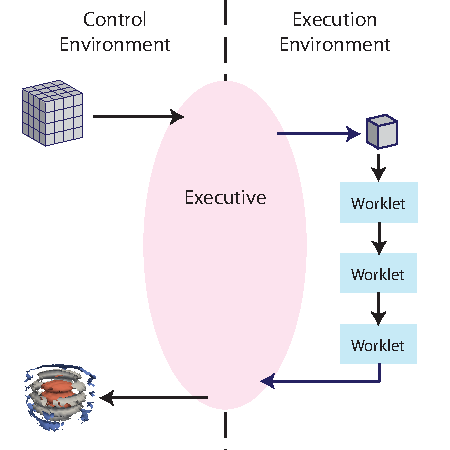
\includegraphics{images/DaxDiagram}
  \caption{Layout of the Dax system.
    Applications using Dax have a different programming and execution environment than the worklets.
    The executive organizes the interaction between these two environments.}
  \label{fig:DaxDiagram}
\end{figure}

The dual programming environments is partially a convenience to isolate the
application from the execution of the worklets and is partially a necessity to
support GPU languages with host and device environments.  The Dax toolkit
provides an object called an \keyterm{Executive} that acts as an interface
between the control and execution environment.  The executive accepts mesh data
and execution requests from the application running in the control environment.
Based on these requests, the executive builds worklet pipelines, manages memory,
and schedules threads in the execution environment.  The relationship between
the control and execution environments and the executive's role in managing them
is demonstrated in Figure~\ref{fig:DaxDiagram}.

\subsection{Data Model}
\label{sec:DataModel}

The data model used by the Dax framework is loosely based on the OpenDX Data Model\lcite{OpenDXManual},
which itself is based on the data model proposed by Haber \etal\scite{Haber1991}.
This data model makes it possible to describe data attributes defined on
different kinds of grids including uniform rectilinear grids, curvilinear grids,
and unstructured grids made up of triangles, quads, tetrahedra, etc. Similar
to OpenDX, the bulk of the data is encapsulated in array objects called
\emph{daxArray}. Also, there are different types of arrays such as
regular array, constant array, and irregular array that make it possible to
compactly represent values in the array. A dataset comprises of a named
collection of arrays with relationships between the arrays. There are two
possible relationships between arrays:
\begin{description}
\item[dep] relationship records a dependency. Array A \emph{dep}ends on
array B implies that A has exactly as many items as B and every item in A
corresponds to an item in B.
\item[ref] relationship records a reference or indirection. Array A
\emph{ref}erences array B implies that values in A are references to values in
B e.g. an array describing the cell connections between points references the
``positions'' array that defines the point coordinates.
\end{description}

\begin{figure}
  \centering
  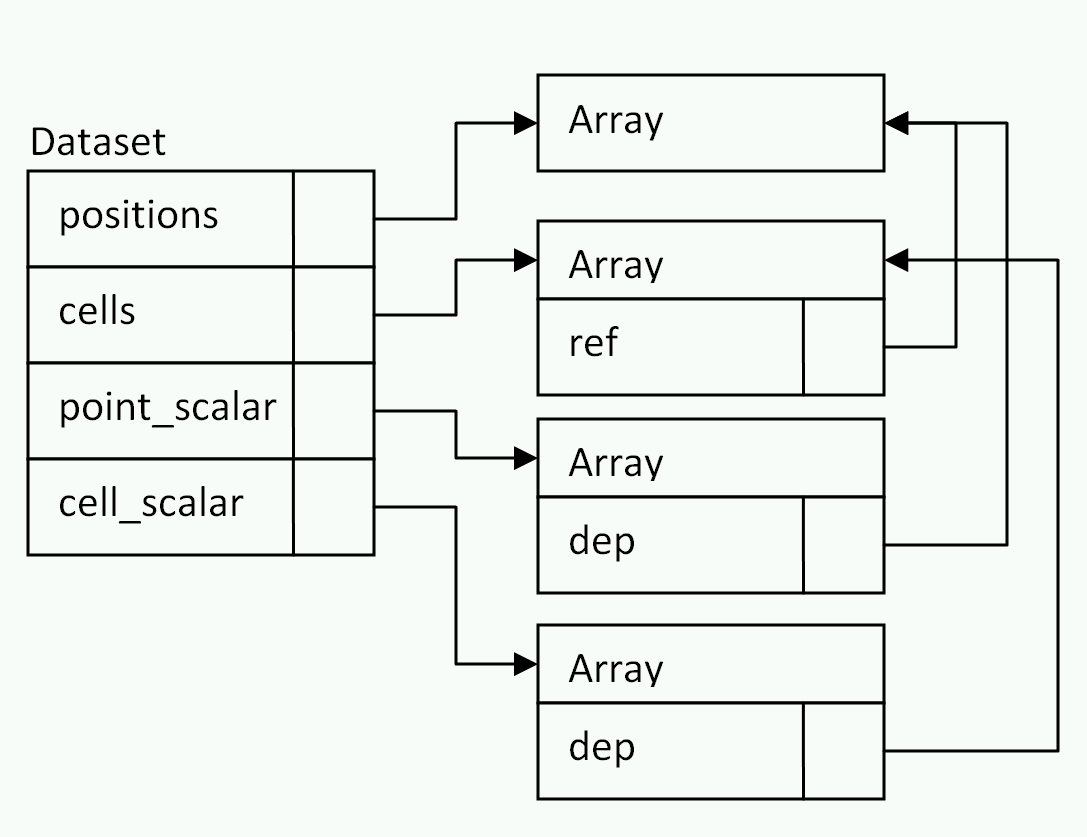
\includegraphics[width=2.5in]{images/DaxDataModel}
  \caption{Example of a dataset with a point and cell scalars.}
  \label{fig:DaxDataModel}
\end{figure}

Figure~\ref{fig:DaxDataModel} shows a representation for a dataset with cell
and point attributes.


\subsection{Execution Model}
\label{sec:ExecutionModel}

The execution model is based on the data-flow paradigm. In a data-flow
implementation, all nodes in the data-flow pipeline are pure stateless functions
through which the data flows. The Dax execution model is similar. It comprises
of Modules (daxModule) that are connected together to form pipelines. The crux
of the module (i.e. the algorithm or the processing logic) is the worklet. A
worklet is C-function that takes processes input array(s) to generate output
array(s). The module can be thought of as the wrapper around the worklet that
facilitates hooking up of these worklets to form pipelines as well as provide
support for type-checking and kernel generation. The Executive
is an object that builds the data-flow pipeline and schedules its execution on
the device. The complexity in the Executive stems from ensuring that the
worklets are executed in correct orders on the device.

For our implementation, we are focusing on OpenCL. Thus the worklet is
written as an OpenCL function using dAPI (Device API) for accessing data
(described later). The executive, accessed via OpenCL's host API,
generates an OpenCL kernel to schedules the kernel for execution to produce
the requested result.

\subsection{Execution Environment}
\label{sec:ExecutionEnvironment}

The worklet code uses this API to access the data, compute values, and then
produce the result. A worklet is a simply a C-function that takes in input
array(s) and produces an output array. The execution environment adds annotations to the arguments
making it possible to deduce relationships between the arguments. For example, the
following code shows the prototype for a worklet that takes in a position
coordinate and point scalar to produce a new point scalar.

\begin{figure}[htbp]
\centering
{\small
\begin{verbatim}
__worklet__ void PointWorklet(daxWork work,
  const daxArray* __positions__ in_positions,
  const daxArray* __dep__(__positions__) in_point_scalars,
  daxArray* __dep__(__positions__) out_scalars)
  {
  daxFloat3 point_cordinate =
    daxGetArrayValue3(work, in_positions);
  daxFloat in_value =
    daxGetArrayValue(work, in_point_scalar);
  daxFloat out_value = ...;
  daxSetArrayValue(work, out_scalars, out_value);
  }
\end{verbatim}
}
\caption{Pseudo-code for a worklet operating on input point scalars and point
coordinates to generate point scalars.}
\label{fig:DaxPointWorklet}
\end{figure}

As is clear from the above code snippet, the worklet code never directly access
any memory locations. It uses the API to get and set values from opaque types. Also,
the datum the operations are being performed on are identified by an opaque
handle called daxWork. \fix{daxWork is kind of confusing given that the name worklet.  Perhaps it could be called something like daxElement.} daxWork makes it possible for the framework to optimize
reads and writes to and from global memory.

The following worklet code computes cell-gradients. It demonstrates
iterating over all the points in a cell and computing a derived quantity, which
is typical of many visualization algorithms.

\begin{figure}[htbp]
\centering
{\small
\begin{verbatim}
__worklet__ void CellGradient(const daxWork work,
  const daxArray* __positions__ in_positions,
  const daxArray*
    __and__(__connections__, __ref__(in_positions))
    in_connections,
  const daxArray* __dep__(in_positions) inputArray,
  daxArray* __dep__(in_connections) outputArray)
{
  daxConnectedComponent cell;
  daxGetConnectedComponent(work, in_connections, &cell);

  daxFloat scalars[MAX_CELL_POINTS];
  uint num_elements = daxGetNumberOfElements(&cell);
  daxWork point_work;
  for (uint cc=0; cc < num_elements; cc++)
    {
    point_work = daxGetWorkForElement(&cell, cc);
    scalars[cc] = daxGetArrayValue(point_work, inputArray);
    }

  daxFloat3 parametric_cell_center =
    (daxFloat3)(0.5, 0.5, 0.5);
  daxFloat3 gradient = daxGetCellDerivative(&cell,
    0, parametric_cell_center, scalars);
  daxSetArrayValue3(work, outputArray, gradient);
}
\end{verbatim} }
\caption{Worklet for computing cell gradients in Dax Execution environment.}
\label{fig:DaxCellGradientWorklet}
\end{figure}

Since the worklet code never directly accesses memory, the framework is free to
optimize the fetches and write-backs to global memory under the covers, avoiding
global memory writes all together for intermediate results in the pipeline.
Furthermore, the design isolates the worklet developers from changes to the
underlying platform. For example, by simply providing CUDA based implementations
for all execution environment and updating the executive to use CUDA runtime components, we
can port the entire framework to a CUDA platform instead of OpenCL.

The annotations used in the arguments to the worklets serve two purposes.
First, it enables the worklet developer to make certain assumptions about
the arrays. For example, if an argument is marked as \emph{\_\_positions\_\_}, the
array represents point coordinates with exactly 3 components.
Second, it enables the control environment (as explained the section \ref{sec:ControlEnvironment}) to validate
the pipeline, catching any invalid connections before the job is dispatched to
the parallel platform.

\subsection{Control Environment}
\label{sec:ControlEnvironment}

The control environment can be considered as the scaffolding interface that helps set up the
visualization pipeline. Each worklet gets wrapped into a module (daxModule),
with each array argument to the worklet becoming an input or an output port for
the module. A pipeline is constructed by connecting the output ports to input
ports on different modules. To execute the pipeline, one calls
Executive::Execute(). That results in first validating the pipeline to ensure
that input port requirements are met. Second, an OpenCL kernel is generated that
executes the entire pipeline on a datum. Finally, the data arrays are
uploaded to the device memory and the OpenCL kernel is triggered.

The execution of the worklets in the pipeline is demand driven. That is, it is
triggered by calling the last worklet in the pipeline. The framework maintains
the information of how each intermediate array is to be generated. When a
worklet makes a daxGetArrayValue\textasteriskcentered~function call, it checks
if the value has been computed or available in global memory. If not, it
executes the source-worklet to produce the value implicitly. Likewise,
daxSetArrayValue\textasteriskcentered~function calls don't necessarily result
in a global memory write. If the array being written to an intermediate result
i.e. result being passed from one worklet to another, then the value gets
written in local memory and returned by the
daxGetArrayValue\textasteriskcentered~ call that triggered the execution of the
worklet. All this is happening under the covers without the worklet having to
worry about any of these optimizations.

Our current implementations don't store any intermediate values. Consequently if
a worklet access the same input array location twice, then the producer worklet
that generates that value is also executed twice. However, based on the
platform, we can easily support sharing of intermediate results between worklet
groups (called workgroups in OpenCL).

\section{Results}
\label{sec:Results}

Table \ref{tab:Results} compares the execution times for a simple pipeline
Elevation $\rightarrow$ Cell Gradient applied to 256x256x256 block of 3D uniform
rectilinear grid using NVIDIA GeForce 8800 GTX graphics card against a serial VTK-based
implementation of the same pipeline on a Intel Xeon 3.00 GHz CPU.

\begin{table}[htbp]
  \centering
  \label{tab:Results}
  \begin{tabular}{|l||c|}
    \hline
    Dax Execution Time & 0.72 s \\
    \hline
    VTK Total Time & 15.61 s \\
    \hline
    \hline
    Speedup & 21.7 \\
    \hline
  \end{tabular}
  \caption{Performance comparison between Dax toolkit and VTK}
\end{table}

We see that even with a simple pipeline involving just two worklets, we can
get a decent speed up.

The code that developer writes in the worklet is comparable to the code
one would write to do the something similar in existing visualization frameworks
such as VTK. Figure~\ref{fig:VTKCellGradient} shows a code snippet for computing
cell gradients in VTK's vtkCellDerivatives filter.

\begin{figure}[htbp]
\centering
{\small
\begin{verbatim}
int vtkCellDerivatives::RequestData(...)
{
  ...[allocate output arrays]...
  ...[validate inputs]...
  for (cellId=0; cellId < numCells; cellId++)
    {
    ...
    input->GetCell(cellId, cell);
    subId = cell->GetParametricCenter(pcoords);
    inScalars->GetTuples(cell->PointIds, cellScalars);
    scalars = cellScalars->GetPointer(0);
    cell->Derivatives(subId, pcoords, scalars, 1, derivs);
    outGradients->SetTuple(cellId, derivs);
    }
  ...[cleanup]...
}
\end{verbatim}
}
\caption{Code to compute cell gradients in VTK (vtkCellDerivatives). Compare
this with code for the same in Dax Toolkit
(Figure~\ref{fig:DaxCellGradientWorklet}).}
\label{fig:VTKCellGradient}
\end{figure}

\section{Challenges Ahead}
\label{sec:Challenges}

In this paper we outlined our proposed framework and demonstrated the
feasibility using worklets that compute point scalars or generate derived cell
quantities using cell geometry and topology. These cover a wide range of
visualization and analysis algorithms however there still remain a set of
algorithms such as clipping cells, iso-surfacing that remain to be addressed. In
general, algorithms that change the topology or connectivity remain to be
handled. The unique characteristic of such algorithms is that they cannot determine the
number of elements a priori. We plan to address this issue using using multiple
passes during the execution stage.


%% It is the visualization and data analysis programmer's responsibility to
%% provide the implementation of a worklet, which describes the behavior of
%% the algorithm.  The Dax toolkit provides the \keyterm{executive}.  The
%% executive applies worklets to data sets.  Like the executive in the VTK
%% pipeline, 

%% VGTC-specific section command.
\acknowledgements{This work was supported in full by the DOE Office of
  Science, Advanced Scientific Computing Research, under award number
  10-014707, program manager Lucy Nowell.

  Part of this work was performed by Sandia National Laboratories.
  Sandia National Laboratories is a multi-program laboratory operated by
  Sandia Corporation, a wholly owned subsidiary of Lockheed Martin
  Corporation, for the U.S. Department of Energy's National Nuclear
  Security Administration.}

\bibliographystyle{abbrv}
\bibliography{DaxLDAV2011}

\end{document}
